\documentclass[11pt,a4paper]{article}

\usepackage[margin=2.2cm]{geometry}
\usepackage{amsmath}
\usepackage{graphicx}
\usepackage{booktabs}
\usepackage{hyperref}
\usepackage{xcolor}

\hypersetup{
    colorlinks=true,
    linkcolor=blue,
    urlcolor=blue
}

\title{Analytical Defence Notes for the 5SC28 Design Project\\
Group 17: Unbalanced Disk Modelling and Control}
\author{Group 17}
\date{\today}

\begin{document}

\maketitle

\section*{Purpose of This Document}

This document is not the final submission report.
It is a preparation document for the presentation and oral defence.
The goal is to explain clearly what the assignment asks, what we did, why we made these choices, and how to answer questions about all parts of the project.
It covers system dynamics modelling, ANN, GP, swing-up control, reference tracking, real setup testing, and submission requirements.

\section{What the Assignment Is About}

The system is an unbalanced disk.
A motor applies a voltage to the system, and the disk angle is measured.
The disk is nonlinear because gravity, inertia, friction, and motor dynamics all affect the motion.
The assignment has three connected objectives:

\begin{itemize}
    \item learn system dynamics models from data using ANN and GP methods;
    \item learn a policy that can swing the disk up to the upright position;
    \item extend the control work so one policy can swing up and track a reference near the upright position.
\end{itemize}

For the modelling part, the assignment gives a very important restriction:

\begin{center}
\textbf{Input: applied motor voltage $u(k)$}\\
\textbf{Output: measured disk angle $\theta(k)$}\\
\textbf{Angular velocity is not used.}
\end{center}

This means the models must learn the relation between voltage history and angle history without directly receiving the angular velocity.
If the model needs information about speed, it must infer it from changes in the measured angle over time.

\subsection*{Overall Project Flow}

The project can be understood as the following chain:

\begin{center}
data $\rightarrow$ dynamics models $\rightarrow$ control policies $\rightarrow$ simulation and real setup testing
\end{center}

The modelling part asks whether we can learn the system behaviour.
The control part asks whether we can use learning methods to make the disk reach useful states.
The final report and defence should explain not only the final numbers, but also why each choice was made and what the limitations are.

\begin{figure}[h]
\centering
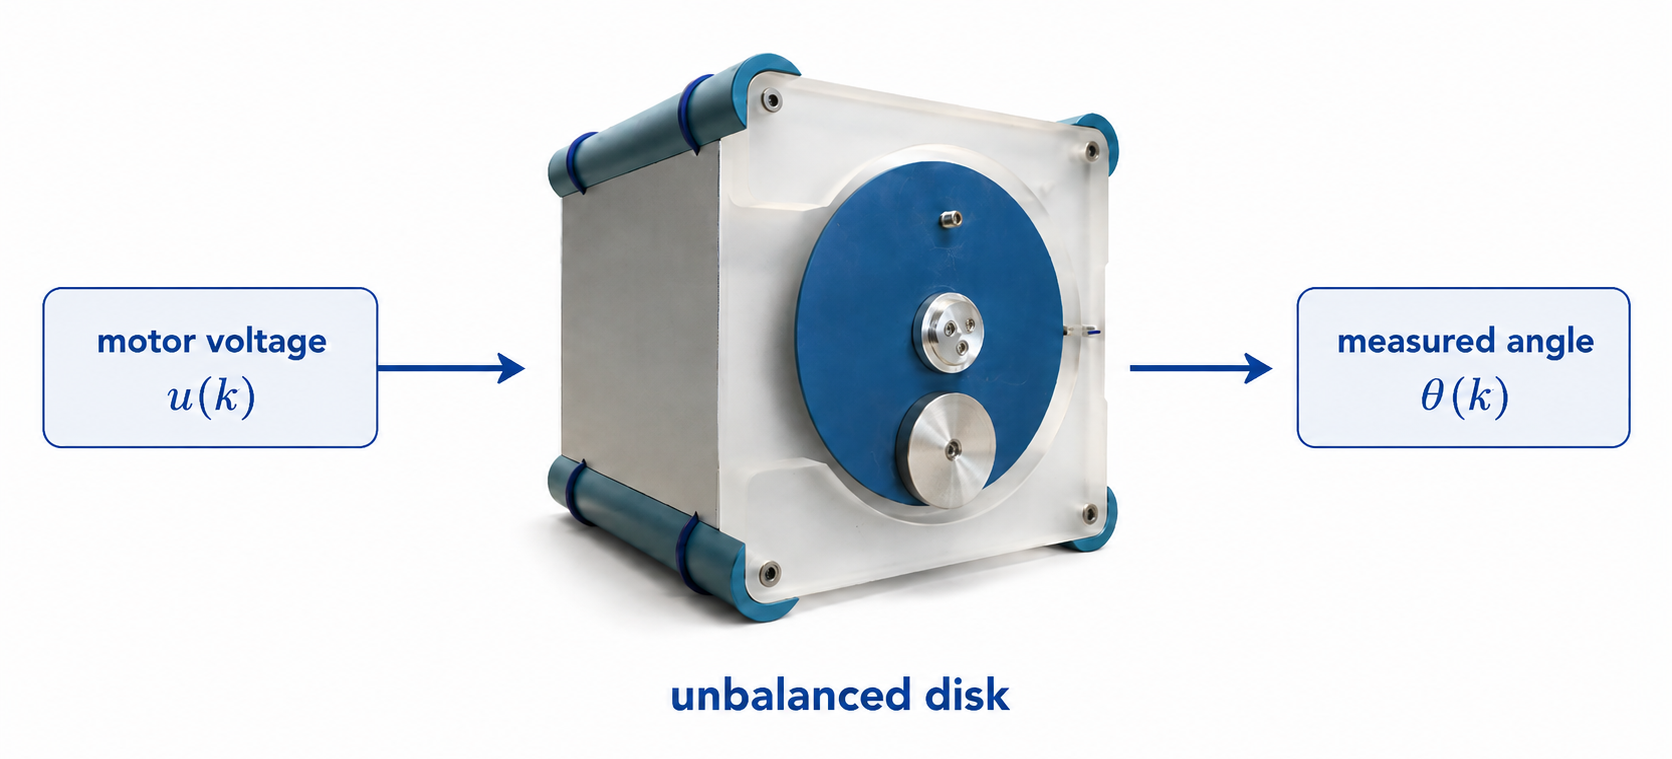
\includegraphics[width=0.95\textwidth]{figures/system_overview.png}
\caption{Input-output view of the unbalanced disk modelling problem.}
\label{fig:system-overview}
\end{figure}

\section{What We Are Trying to Learn}

The modelling task is system identification.
In simple words, we want a mathematical or machine-learning model that behaves like the real system.
The model should receive voltage and past angle information, and it should predict the next disk angle or simulate a full angle trajectory.

The general modelling idea is

\begin{equation}
\hat{\theta}(k) = f(\text{past voltages}, \text{past angles}),
\end{equation}

where $\hat{\theta}(k)$ is the model output and $\theta(k)$ is the measured disk angle from the dataset.

This is needed because the disk has memory.
The next angle is not determined only by the current voltage.
The same voltage can lead to different motion depending on where the disk was and how it was moving before.
Because angular velocity is not used directly, past angle samples are especially important.

\section{Prediction and Simulation}

The assignment asks us to validate models using both prediction and simulation.
These are not the same thing.

\subsection{Prediction}

Prediction means one-step-ahead prediction.
The model predicts the next angle using measured previous angles.
This is the easier task because the model is corrected at every step by the true measured past data.

In prediction, if the model makes a small mistake at sample $k$, that mistake does not strongly affect sample $k+1$, because the next input still contains measured data from the real system.

The question answered by prediction is:

\begin{center}
\textit{Given the real recent history, can the model predict the next angle accurately?}
\end{center}

\subsection{Simulation}

Simulation means generating a full trajectory.
After a short measured starting part, the model uses its own previous predicted angles as inputs.
This is harder because errors can accumulate.

In simulation, if the model is slightly wrong at one sample, that wrong value becomes part of the input for the next sample.
Therefore, simulation tests whether the model has really learned stable dynamics.

The question answered by simulation is:

\begin{center}
\textit{Can the model reproduce the system behaviour over time when it has to rely on itself?}
\end{center}

\subsection{Why Both Are Needed}

A model can be good at prediction but bad at simulation.
This happened in our comparison: the GRU had the best prediction error, while the LSTM had the best simulation error.
This is why both tasks are important.
Prediction checks local one-step accuracy.
Simulation checks long-term dynamic behaviour.

\section{Error Measure: RMSE}

The error metric used in our ANN comparison is the root mean squared error (RMSE):

\begin{equation}
\mathrm{RMSE} =
\sqrt{\frac{1}{N}\sum_{k=1}^{N}\left(\theta(k)-\hat{\theta}(k)\right)^2}.
\end{equation}

Here:

\begin{itemize}
    \item $\theta(k)$ is the measured disk angle from the dataset;
    \item $\hat{\theta}(k)$ is the model output;
    \item $N$ is the number of evaluated samples.
\end{itemize}

RMSE is useful because it gives one number for the typical size of the error.
We report it in degrees because degrees are easier to interpret than radians.

\section{The ANN Part}

The ANN part required at least:

\begin{itemize}
    \item one simple ANN model;
    \item one more advanced ANN architecture.
\end{itemize}

We compared three ANN models:

\begin{itemize}
    \item simple NARX feedforward ANN;
    \item advanced GRU recurrent ANN;
    \item advanced LSTM recurrent ANN.
\end{itemize}

\subsection{Why We Used a NARX Model}

NARX means nonlinear autoregressive model with exogenous input.
In this project, that means the model predicts the next angle using old motor voltages and old measured angles:

\begin{equation}
\hat{\theta}(k) =
f_{\mathrm{ANN}}(u(k-15), \ldots, u(k-1),
\theta(k-15), \ldots, \theta(k-1)).
\end{equation}

This was a good simple baseline for four reasons.

\begin{itemize}
    \item It uses only allowed signals: voltage and measured angle.
    \item It includes memory through delayed samples.
    \item It is simple and close to practical-session model structures.
    \item It gives a fair baseline to see whether advanced recurrent models are actually better.
\end{itemize}

We did not use only the current voltage because the system has memory.
We also did not start only with LSTM because then we would not have a simple baseline.

\subsection{Why We Used GRU and LSTM}

GRU and LSTM are recurrent neural networks.
They are designed for sequence data.
This is useful here because the unbalanced disk is a dynamical system, so the order of previous samples matters.

Both recurrent models use sequence inputs of the form

\begin{equation}
[(u(k-H),\theta(k-H)), \ldots, (u(k-1),\theta(k-1))]
\rightarrow \hat{\theta}(k),
\end{equation}

with history length $H=15$.

The reason for testing both GRU and LSTM is that they have different complexity.
The GRU is simpler and has fewer gates.
It can train well and often gives strong one-step prediction performance.
The LSTM has a more detailed memory mechanism.
This can help when longer-term stability matters, especially in simulation.

\subsection{Training Method}

All ANN models were trained using supervised learning.
The training target was the measured next angle from the dataset.
The model output was compared with the measured angle, and the model weights were adjusted to reduce the mean squared error.

The optimizer used was Adam.
Adam is not a model.
It is the algorithm that updates the neural-network weights during training.
In simple words:

\begin{center}
prediction $\rightarrow$ error $\rightarrow$ update weights $\rightarrow$ smaller error
\end{center}

The data were split into:

\begin{itemize}
    \item 70 percent training data;
    \item 15 percent validation data;
    \item 15 percent test data.
\end{itemize}

The validation data helped with model selection.
The test data were used to compare the final models.

\section{ANN Results and Interpretation}

\begin{table}[h]
\centering
\caption{ANN validation results on the held-out test split.}
\begin{tabular}{lcc}
\toprule
Model & Prediction RMSE & Simulation RMSE \\
\midrule
Simple NARX ANN & 2.442 deg & 16.130 deg \\
Advanced GRU ANN & 0.202 deg & 2.031 deg \\
Advanced LSTM ANN & 0.235 deg & 1.893 deg \\
\bottomrule
\end{tabular}
\end{table}

\begin{figure}[h]
\centering
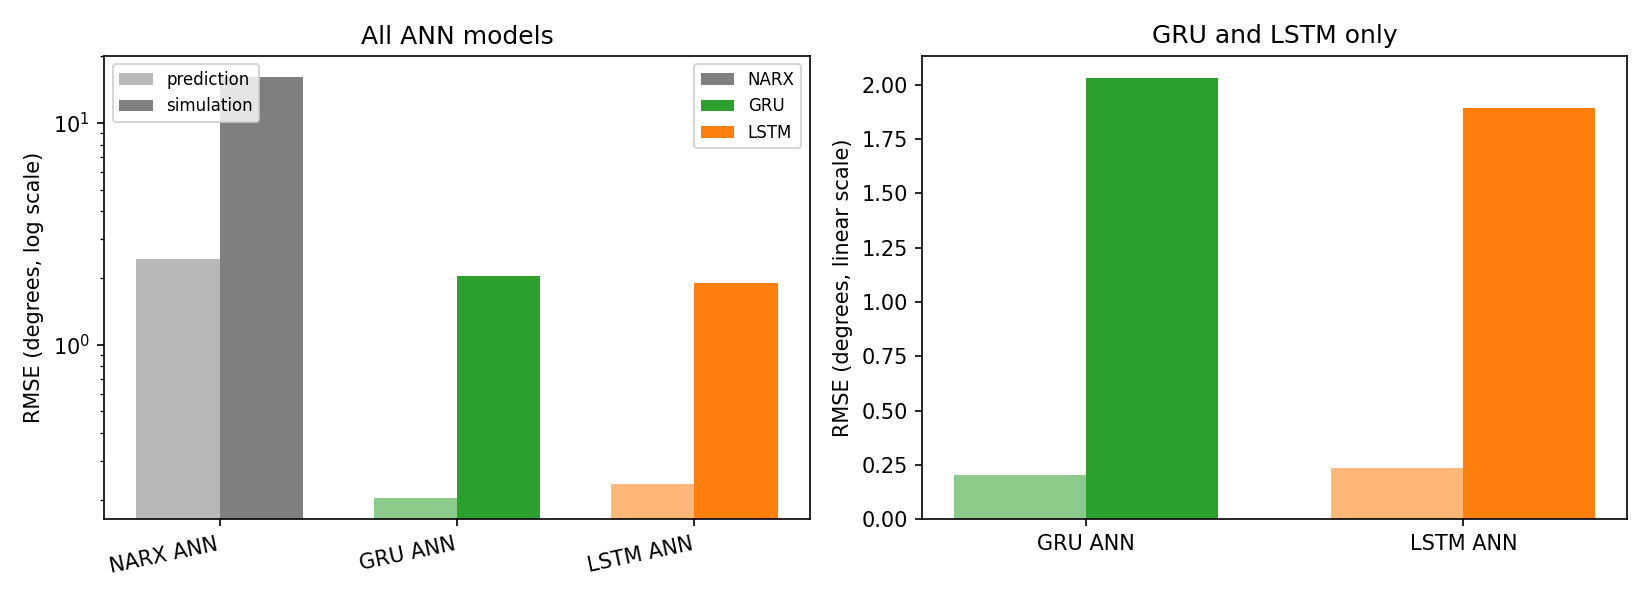
\includegraphics[width=0.95\textwidth]{figures/ann_three_model_comparison.png}
\caption{ANN prediction and simulation comparison.}
\label{fig:ann-comparison}
\end{figure}

\subsection{What the Numbers Mean}

The simple NARX model has much worse simulation error.
This means it can learn some local input-output relation, but it does not capture the long-term dynamics well enough.

The GRU gives the best prediction result.
This means it is very good at the one-step task when measured past angles are available.

The LSTM gives the best simulation result.
This means it is slightly better when the model must feed back its own predictions over time.
Since simulation is harder and more important for checking learned dynamics, the LSTM was selected as the final ANN model.

\subsection{Why GRU Prediction Is Better but LSTM Simulation Is Better}

Prediction and simulation test different behaviour.
In prediction, the model receives measured past angles.
The task is mainly to fit the next-step relation.
The simpler GRU can do this very well.

In simulation, the model receives its own previous predictions.
Small errors can feed back into the model and grow over time.
The LSTM memory mechanism appears to be slightly more stable for this longer trajectory task.

This is an important defence point:

\begin{center}
\textbf{Best prediction model does not automatically mean best simulation model.}
\end{center}

\section{Understanding the Error Spike Around Sample 400}

In the simulation error plot, there is a temporary error increase around sample 400.
This happens because the measured angle changes quickly in that region.
During fast transient motion, a small timing difference between the model and the measured system produces a visible error.

This is expected because angular velocity is not used as an input.
The model must infer speed from previous angle samples.
That works reasonably well, but it is not perfect during fast changes.

A good oral answer is:

\begin{quote}
The spike happens during a fast change in the disk angle. Since the model does not directly use angular velocity, it must infer the speed from previous angle samples. A small delay or timing mismatch then becomes visible as a temporary error peak.
\end{quote}

\section{The GP Modelling Part}

The GP model is the second required system dynamics model.
It uses the same assignment input-output rule as the ANN models:

\begin{center}
past motor voltage and past measured angle $\rightarrow$ next angle behaviour
\end{center}

The final GP folder describes the selected model as a sparse delta-output GP-NARX model.
This means the GP does not directly predict the full next angle.
Instead, it predicts the change in angle:

\begin{equation}
\Delta \theta(k) = \theta(k) - \theta(k-1).
\end{equation}

The next angle is then reconstructed as

\begin{equation}
\hat{\theta}(k) = \theta(k-1) + \widehat{\Delta \theta}(k).
\end{equation}

\subsection{Why Use a Delta-Output GP?}

Predicting $\Delta \theta$ can be easier than predicting the full angle directly.
The model learns the local change in the system instead of the absolute angle value.
This can improve simulation behaviour because the simulated trajectory is built up step by step.

\subsection{Why Use a Sparse GP?}

A normal GP can become computationally expensive when there are many training samples.
This is because GP training involves matrix operations that scale poorly with the number of data points.
A sparse GP uses a smaller set of inducing points to approximate the full GP.
This reduces computational cost while keeping the useful uncertainty and nonlinear modelling behaviour of a GP.

\subsection{Final GP Structure}

The final GP setting in the project files was:

\begin{itemize}
    \item model type: GPy sparse delta-output GP-NARX;
    \item output: $\Delta \theta$;
    \item past angle order: $n_a = 10$;
    \item past input order: $n_b = 8$;
    \item inducing points: $M = 250$;
    \item kernel: Matern 5/2.
\end{itemize}

The GP input dimension was therefore 18, because it used 10 past angle terms and 8 past voltage terms.

\subsection{GP Results}

The validation results stored in the GP folder are:

\begin{table}[h]
\centering
\caption{Final GP validation results.}
\begin{tabular}{lc}
\toprule
Metric & Value \\
\midrule
Prediction RMSE & 0.1638 deg \\
Simulation RMSE & 1.4615 deg \\
Simulation NRMS & 5.04 percent \\
\bottomrule
\end{tabular}
\end{table}

The GP result is slightly better than the final ANN result on our validation split.
For comparison, the LSTM ANN simulation RMSE was 1.893 deg, while the GP simulation RMSE was 1.4615 deg.

\subsection{How to Explain GP vs ANN}

A good defence answer is:

\begin{quote}
Both ANN and GP models learn nonlinear dynamics from the same allowed signals: voltage and measured angle.
The ANN models are flexible neural-network models trained by gradient descent.
The GP model is probabilistic and kernel-based.
In our validation results, the sparse delta-output GP gave the best modelling RMSE, while the LSTM was the best ANN model.
\end{quote}

Important limitation:
the trained GP model files were too large to store directly in the GitHub folder, so the final GP output files are included, but full rerunning may require the separate local model file.

\section{The Swing-Up Control Part}

The second major assignment objective is to learn a policy that swings the disk from the stable bottom position to the unstable upright position.

A policy is a rule that maps the current state or observation to an action:

\begin{equation}
a(k) = \pi(s(k)).
\end{equation}

Here, $s(k)$ is the state or observation used by the controller, and $a(k)$ is the selected action.
In this system, the action corresponds to applying a motor voltage.

\subsection{What Makes Swing-Up Hard?}

The upright position is unstable.
The controller cannot simply move there slowly and stop.
It must inject energy into the disk, swing it up, and then stabilize it near the top.

The voltage is also limited.
Therefore, the controller must learn when to use strong actions and when to reduce the input near the target.

\subsection{DQN / Q-Learning Style Controller}

The project contains a DQN/Q-learning swing-up controller.
The basic reinforcement-learning idea is:

\begin{itemize}
    \item the controller observes the current situation;
    \item it chooses an action;
    \item it receives a reward;
    \item training tries to learn actions that maximize long-term reward.
\end{itemize}

The Q-function estimates how good an action is in a given state:

\begin{equation}
Q(s,a) \approx \text{expected future reward after taking action } a \text{ in state } s.
\end{equation}

A DQN uses a neural network to approximate this Q-function.

The best DQN swing-up evaluation file reports:

\begin{table}[h]
\centering
\caption{DQN swing-up result from the stored evaluation metrics.}
\begin{tabular}{lc}
\toprule
Metric & Value \\
\midrule
Success & true \\
Final error & 0.0374 rad \\
Last-window mean absolute error & 0.0374 rad \\
Upright ratio & 0.9233 \\
Maximum input & 3.0 V \\
Saturation ratio & 0.0733 \\
\bottomrule
\end{tabular}
\end{table}

This means the DQN policy succeeded in simulation and spent most of the episode close to the upright position.

\subsection{Hybrid / Model-Internalization Style Controller}

The project also contains a hybrid policy/model-internalization style controller.
The folder description says it includes teacher data, RBF imitation, hybrid policy optimization, and robustness evaluation.

The idea is different from pure DQN.
Instead of only learning an action-value function, the method combines simpler control ideas and learned/imitation components.
The final optimized hybrid policy improved the initial hybrid policy.

Stored metrics show:

\begin{table}[h]
\centering
\caption{Optimized hybrid swing-up result.}
\begin{tabular}{lc}
\toprule
Metric & Value \\
\midrule
Final error & 0.0115 rad \\
Last-window mean absolute error & 0.0131 rad \\
Upright ratio & 0.8467 \\
Maximum input & 2.7481 V \\
Saturation ratio & 0.0 \\
\bottomrule
\end{tabular}
\end{table}

The robustness evaluation reports a success rate of 1.0 over 50 episodes.
This is important because it suggests the policy is not only successful in one lucky run.

\subsection{How to Explain the Swing-Up Control Results}

A good defence answer is:

\begin{quote}
The swing-up task was evaluated by checking whether the disk reached and stayed near the upright position.
The DQN policy succeeded and had a high upright ratio.
The optimized hybrid policy also succeeded and avoided voltage saturation in the stored evaluation.
The robustness test for the optimized hybrid policy showed success over multiple episodes, which is useful evidence that the result was not just one lucky trajectory.
\end{quote}

\section{The Reference Tracking Part}

The third assignment objective is to extend the controller so that one policy can both swing up and track a reference near the upright position.

This is harder than simple swing-up because the goal is no longer only:

\begin{center}
reach upright and stay there
\end{center}

The goal becomes:

\begin{center}
reach upright and follow a changing reference signal
\end{center}

\subsection{What Reference Tracking Measures}

The tracking error is the difference between the disk angle and the reference angle:

\begin{equation}
e(k) = \theta(k) - \theta_{\mathrm{ref}}(k).
\end{equation}

A good tracking controller should keep this error small while respecting voltage limits.

\subsection{Stored Reference-Tracking Result}

The reference-tracking folder contains a DQN reference-tracking controller and stored evaluation metrics.
The representative evaluation reports:

\begin{table}[h]
\centering
\caption{Representative DQN reference-tracking result.}
\begin{tabular}{lc}
\toprule
Metric & Value \\
\midrule
Success & true \\
Final error & -0.0425 rad \\
Last-window mean absolute error & 0.0459 rad \\
Tracking ratio & 0.9167 \\
Maximum input & 3.0 V \\
Saturation ratio & 0.0867 \\
\bottomrule
\end{tabular}
\end{table}

This suggests the learned reference-tracking policy can both reach the useful operating region and follow the reference for most of the evaluation.

\subsection{How to Explain Reference Tracking}

A good defence answer is:

\begin{quote}
Swing-up only asks the controller to reach the upright region.
Reference tracking asks the controller to keep following a desired angle near the upright position.
Therefore, the reward and evaluation must include tracking error, not only whether the disk is upright.
\end{quote}

\section{Real Setup Testing}

The professor announcement says the oral defence will discuss the results, implementation, and theory.
The real setup is important because simulation and physical behaviour can differ.

If the teammate runs real setup tests, the report should record:

\begin{itemize}
    \item test date and controller version;
    \item number of trials;
    \item initial condition;
    \item voltage limits and safety checks;
    \item measured angle and voltage logs;
    \item whether the trial succeeded;
    \item differences between simulation and real setup.
\end{itemize}

Possible reasons why real behaviour can differ from simulation:

\begin{itemize}
    \item friction is not modelled perfectly;
    \item sensor noise;
    \item time delays;
    \item voltage saturation;
    \item model mismatch;
    \item different initial conditions.
\end{itemize}

A good defence answer is:

\begin{quote}
The real setup is the final test of whether the learned policy transfers from simulation.
Even if performance is worse than in simulation, this is useful because it reveals practical issues such as friction, noise, delay, and saturation.
\end{quote}

\section{Submission Requirements}

The announcement says the group submission should include:

\begin{itemize}
    \item a design assignment report in IEEE two-column format, 6--12 pages;
    \item a folder with requested prediction and simulation test files;
    \item a folder with relevant code and additional material.
\end{itemize}

For the modelling files, the submission should include at least:

\begin{itemize}
    \item one ANN prediction result;
    \item one ANN simulation result;
    \item one GP prediction result;
    \item one GP simulation result.
\end{itemize}

\section{Likely Oral Defence Questions and Answers}

\subsection*{What is the input and output of the modelling problem?}

The input is the applied motor voltage $u(k)$.
The output is the measured disk angle $\theta(k)$.
Angular velocity is not used because the assignment explicitly says not to use it.

\subsection*{How do we know the real measured angle?}

It is included in the provided dataset.
The dataset contains the measured angle signal, usually stored as \texttt{th}.
This is used as the reference when calculating model error.

\subsection*{Why do we use delayed samples?}

The disk is dynamic.
The next angle depends on previous voltages and previous angles, not only on the current voltage.
Delayed samples give the model memory.

\subsection*{Why NARX?}

NARX is a simple dynamic model structure.
It uses previous outputs and previous inputs.
It is simple enough to be a baseline, but still meaningful for a dynamical system.

\subsection*{Why recurrent neural networks?}

GRU and LSTM are built for sequence data.
They process the order of past voltage and angle values more naturally than a feedforward network.
This is useful because the unbalanced disk has time-dependent dynamics.

\subsection*{What is the difference between GRU and LSTM?}

Both are recurrent models.
GRU is simpler and has fewer gates.
LSTM has a more detailed memory mechanism.
In our results, GRU was slightly better for one-step prediction, while LSTM was slightly better for simulation.

\subsection*{Why is simulation harder than prediction?}

Prediction uses measured past angles.
Simulation uses the model's own previous predicted angles.
Therefore, simulation errors can accumulate over time.

\subsection*{Why did we choose LSTM as the final ANN output?}

The LSTM had the lowest simulation RMSE.
Simulation is the harder test and better checks whether the model learned stable system dynamics.

\subsection*{Why is RMSE reported in degrees?}

The model works with angles, and degrees are easier to interpret than radians.
The calculation is first done in radians and then converted to degrees using

\begin{equation}
\mathrm{error}_{deg} = \frac{\mathrm{error}_{rad}}{2\pi}360.
\end{equation}

\subsection*{What is Adam?}

Adam is the optimizer used to train the neural networks.
It updates the model weights to reduce the loss.
It is not the neural network itself.

\subsection*{What are the limitations of the ANN work?}

The main limitations are:

\begin{itemize}
    \item limited hyperparameter tuning;
    \item no angular velocity input;
    \item recurrent models are less interpretable than a simple NARX model;
    \item results are based on the available validation/test split, while hidden test performance is not known during development.
\end{itemize}

\subsection*{What is the difference between ANN and GP modelling?}

Both learn nonlinear system dynamics from data.
The ANN is a neural-network function approximator trained by minimizing a loss.
The GP is a kernel-based probabilistic model.
The GP can provide a more structured way to model uncertainty, while the ANN can scale well and is flexible.
In our validation results, the sparse delta-output GP had the lowest modelling RMSE.

\subsection*{Why did the GP predict delta angle instead of angle directly?}

Predicting $\Delta\theta$ means predicting the local change in angle.
This can be easier because the model learns how the state changes from one step to the next.
The full angle is then reconstructed by adding the predicted change to the previous angle.

\subsection*{Why was a sparse GP used?}

A full GP can become slow with many data points because it requires expensive matrix computations.
A sparse GP uses inducing points to approximate the full GP.
This makes training and prediction more practical.

\subsection*{What does the Matern 5/2 kernel do?}

The kernel defines how the GP measures similarity between input points.
A Matern 5/2 kernel is commonly used for smooth but not overly smooth functions.
That is suitable for physical dynamics because the system response is continuous but not perfectly simple.

\subsection*{What is a policy?}

A policy is a rule that maps a state or observation to an action.
For this project, the action is related to the motor voltage.

\subsection*{What is the difference between modelling and control?}

Modelling asks: can we predict how the system behaves?
Control asks: can we choose inputs so the system does what we want?
The modelling part evaluates prediction and simulation accuracy.
The control part evaluates task success, tracking error, voltage usage, and robustness.

\subsection*{What is DQN?}

DQN means Deep Q-Network.
It uses a neural network to approximate the Q-function, which estimates the long-term value of taking an action in a state.
The controller chooses actions based on these learned values.

\subsection*{What is the reward function for?}

The reward function tells the reinforcement-learning algorithm what behaviour is good.
For swing-up, good behaviour means reaching and staying near upright.
For reference tracking, good behaviour means staying close to the reference while using acceptable control effort.

\subsection*{Why is reference tracking harder than swing-up?}

Swing-up mainly requires reaching the upright region.
Reference tracking requires reaching the upright region and then following a changing desired angle.
So the controller must both stabilize and track.

\subsection*{Why do we care about saturation ratio?}

Saturation ratio tells how often the controller uses the maximum allowed voltage.
A lower saturation ratio usually means smoother control and more margin for the real system.
If the controller is always saturated, it may be less robust.

\subsection*{What should we say if real setup results differ from simulation?}

That is expected.
Simulation is an approximation.
Real hardware includes friction, sensor noise, time delay, actuator limits, and unmodelled effects.
A good report should discuss these differences honestly instead of hiding them.

\section{Short ANN Presentation Script}

For my part, I focused on ANN modelling of the system dynamics.
The input to the model is the applied motor voltage, and the output is the measured disk angle.
Angular velocity was not used, following the assignment.

I compared three ANN models.
The first was a simple NARX feedforward network, which uses delayed voltages and delayed angles.
This was used as a baseline.
Then I tested two recurrent models, a GRU and an LSTM, because the disk data is sequential and the order of previous samples matters.

The models were evaluated using prediction and simulation.
Prediction is one-step-ahead and uses measured past angles.
Simulation is harder because the model feeds back its own previous predictions.

The results showed that both recurrent models performed much better than the simple NARX network.
The GRU had the best prediction RMSE, while the LSTM had the best simulation RMSE.
Because simulation is the more demanding test of learned dynamics, the LSTM was selected as the final ANN model.

\end{document}
